\documentclass[a4paper,12pt]{report}

% Paquetes necesarios
\usepackage[utf8]{inputenc}   % Codificación UTF-8
\usepackage{fontspec} % Paquete para manejar fuentes específicas
\usepackage[spanish]{babel}
\usepackage[style=apa, backend=biber]{biblatex}
\usepackage{geometry}         % Configuración de márgenes
\usepackage{graphicx}
\usepackage{setspace}         % Configuración de interlineado
\usepackage{fancyhdr}         % Configuración de encabezados y pie de página
\usepackage{titlesec} % Para personalizar títulos de capítulos
\usepackage{hyperref} % Opcional: Para hipervínculos en el índice
\usepackage{enumitem}
\usepackage{placeins}



\setmainfont{Arial}   % Configura Arial como la fuente principal
\geometry{
    top=2.5cm,
    bottom=2.5cm,
    left=4cm,
    right=2.5cm
}
\pagestyle{fancy}
% Configuración del interlineado y espacio entre párrafos
% \setlength{\parskip}{2em}  % Espacio doble entre párrafos
% \setlength{\parindent}{0em} % Sin sangría en párrafos
\onehalfspacing            % Interlineado de 1.5
% Configuración del pie de página
\fancyhf{}
\fancyfoot[R]{\thepage}    % Número de página en la esquina inferior derecha
\fancypagestyle{plain}{
    \fancyhf{}
    \fancyfoot[R]{\thepage}
}

% Configuración para personalizar capítulos sin la palabra "Capítulo"
\newcommand{\customchapter}[1]{
    \chapter*{#1} % Capítulo sin "Capítulo" y sin numeración
    % \addcontentsline{toc}{chapter}{#1} % Agrega al índice sin numerar
}

% Configuración para personalizar títulos de capítulos específicos
\newcommand{\nochapterlabel}{
  \titleformat{\chapter}[hang]
    {\normalfont\huge\bfseries}
    {\thechapter.}{1em}{} % Quita "Capítulo" pero deja el número
}


\addbibresource{bibliography.bib} % Archivo .bib con las referencias



\begin{document}

% Incluir la portada
% Archivo: portada.tex
\begin{titlepage}
    \begin{center}
        {\fontsize{15pt}{10pt}\selectfont\textbf{UNIVERSIDAD AUTÓNOMA "GABRIEL RENE MORENO"}} \\
        {\fontsize{15pt}{10pt}\selectfont\textbf{FACULTAD DE INGENIERÍA EN CIENCIAS DE LA COMPUTACIÓN Y TELECOMUNICACIONES}} \\
        \vspace{1cm}
        % Logo
        
\includegraphics[width=0.8\textwidth]{images/logo_soe.png} \\
        
        % Título de la institución
        {\fontsize{15pt}{10pt}\selectfont\textbf{MAESTRÍA EN CIENCIA DE DATOS E INTELIGENCIA ARTIFICIAL}} \\

        % Título del trabajo
        \vspace{1cm}
        {\fontsize{15pt}{5pt}\selectfont\textbf{Implementar un Chatbot Semántico Multiperfil para Acceso Inteligente a Documentación Técnica y de Negocio en Plataformas Confluence del Sector Aeronáutico en Airnguru S.A. para la Gestión 2025}} \\
        \vspace{1cm}
        
        \vspace{2cm}
        \begin{flushright}
        {\fontsize{14pt}{22pt}\selectfont\textbf{Autor}} \\
        {\fontsize{14pt}{22pt}\selectfont{Ing. Darlyn Bravo Peña}} \\
        \end{flushright}
        
        
        
        % Ciudad y fecha
        \vfill
        \textbf{Santa Cruz, Bolivia} \\
    \end{center}
    \end{titlepage}
     % Reemplaza con % Archivo: portada.tex
\begin{titlepage}
    \begin{center}
        {\fontsize{15pt}{10pt}\selectfont\textbf{UNIVERSIDAD AUTÓNOMA "GABRIEL RENE MORENO"}} \\
        {\fontsize{15pt}{10pt}\selectfont\textbf{FACULTAD DE INGENIERÍA EN CIENCIAS DE LA COMPUTACIÓN Y TELECOMUNICACIONES}} \\
        \vspace{1cm}
        % Logo
        
\includegraphics[width=0.8\textwidth]{images/logo_soe.png} \\
        
        % Título de la institución
        {\fontsize{15pt}{10pt}\selectfont\textbf{MAESTRÍA EN CIENCIA DE DATOS E INTELIGENCIA ARTIFICIAL}} \\

        % Título del trabajo
        \vspace{1cm}
        {\fontsize{15pt}{5pt}\selectfont\textbf{Implementar un Chatbot Semántico Multiperfil para Acceso Inteligente a Documentación Técnica y de Negocio en Plataformas Confluence del Sector Aeronáutico en Airnguru S.A. para la Gestión 2025}} \\
        \vspace{1cm}
        
        \vspace{2cm}
        \begin{flushright}
        {\fontsize{14pt}{22pt}\selectfont\textbf{Autor}} \\
        {\fontsize{14pt}{22pt}\selectfont{Ing. Darlyn Bravo Peña}} \\
        \end{flushright}
        
        
        
        % Ciudad y fecha
        \vfill
        \textbf{Santa Cruz, Bolivia} \\
    \end{center}
    \end{titlepage}
     si prefieres que se trate como una sección independiente

% Table of contents
\newpage
\tableofcontents
\newpage
\listoffigures
\newpage
\begin{center}
    {\LARGE \textbf{INTRODUCCIÓN}} % Título centrado y en negrita
\end{center}

La estimación de costos en el desarrollo de software es un desafío inherente a la naturaleza intangible de este producto. En un mundo donde la economía digital impulsa la innovación y la competitividad, la incapacidad de calcular con precisión los costos de desarrollo puede llevar a pérdidas financieras, proyectos fallidos y relaciones comerciales insatisfactorias. A nivel global, empresas de todos los tamaños enfrentan la necesidad de establecer modelos más eficientes y estandarizados para valorar su trabajo, especialmente en un mercado donde la externalización y la globalización son cada vez más comunes. Este tema adquiere mayor relevancia 
con el auge de las metodologías ágiles y la inteligencia artificial, que prometen pero también complican la predicción de costos.

En Bolivia, donde el sector tecnológico está en crecimiento, el problema de la estimación de costos en el desarrollo de software adquiere un matiz especial. La falta de modelos estandarizados y herramientas locales para valorar los servicios de desarrollo de software lleva a una alta dependencia de las negociaciones subjetivas, lo que puede perjudicar tanto a los desarrolladores como a los clientes. Esto es especialmente importante en un contexto donde muchas empresas están comenzando a digitalizarse y dependen del software para competir en un mercado nacional e internacional. Abordar este desafío no solo contribuirá al fortalecimiento del sector tecnológico en Bolivia, sino que también permitirá que los desarrolladores y empresas logren acuerdos más justos y sostenibles, impulsando así el crecimiento de la economía digital en el país.

El tema está ubicado en el area 
Ciencias Generales de la Computación Aplicadas y la 
línea Ingeniería de software con un eje de 
Aspectos económicos y de negocio del proceso de desarrollo del software porque la estimación de costos afecta la 
rentabiliad de los proyectos del software, tanto para los desarrolladores
como para los clientes.
\section{Antecedentes}
La estimación precisa de costos en el desarrollo de software es un desafío constante en la ingeniería de software, especialmente en entornos ágiles. Técnicas como los \textit{Puntos de Historia} y el \textit{Planning Poker} han sido desarrolladas para abordar este problema, permitiendo a los equipos estimar el esfuerzo necesario para completar historias de usuario de manera colaborativa 
y basada en consenso \parencite{asana_planning_poker}
Los \textit{Puntos de Historia} son una unidad de medida abstracta que refleja el esfuerzo relativo, la complejidad y el riesgo asociados a una historia de usuario. Esta técnica permite a los equipos evaluar tareas en función de su tamaño relativo, en lugar de estimar en unidades de tiempo, lo que facilita 
la planificación y priorización en entornos ágiles \parencite{asana_story_points}.

Por otro lado, el \textit{Planning Poker} es una técnica de estimación que combina la opinión de todos los miembros del equipo para alcanzar una estimación consensuada. Durante una sesión de \textit{Planning Poker}, cada miembro selecciona de manera independiente una carta con el valor que considera adecuado para una tarea específica. Posteriormente, las discrepancias se discuten hasta alcanzar un consenso, promoviendo 
la colaboración y la precisión en las estimaciones \parencite{asana_planning_poker}.

A pesar de su efectividad en proyectos ágiles, estas técnicas enfrentan desafíos, como la subjetividad inherente al proceso y la falta de estandarización en algunos equipos. Sin embargo, su uso ha demostrado ser fundamental para mejorar la precisión de las estimaciones y la planificación 
en proyectos de software de diversa escala \parencite{asana_planning_poker}.

\section{Presentación de las Problemáticas}

El enfoque ágil, específicamente mediante técnicas como los \textit{puntos de historia} y el \textit{Planning Poker}, busca mejorar la precisión en las estimaciones promoviendo la colaboración entre equipos y utilizando métricas iterativas y relativas. Sin embargo, estas metodologías enfrentan problemáticas clave, como:

\begin{itemize}
    \item \textbf{Subjetividad en las estimaciones:} Las valoraciones basadas en puntos de historia pueden variar significativamente según la experiencia y perspectiva de los miembros del equipo.
    \item \textbf{Dependencia de la experiencia del equipo:} La efectividad de \textit{Planning Poker} depende de un equipo con experiencia previa en proyectos similares, lo que limita su aplicabilidad en equipos menos maduros.
    \item \textbf{Dificultad en la estandarización:} Los puntos de historia y \textit{Planning Poker} no siempre son fácilmente comparables entre equipos o proyectos, lo que complica la evaluación del desempeño y la predicción futura.
    \item \textbf{Falta de datos históricos:} En proyectos nuevos o innovadores, la ausencia de datos históricos dificulta establecer referencias confiables para las estimaciones.
\end{itemize}


\section{Situación Problemática}

La estimación de costos y tiempos en el desarrollo de software es un componente crítico para garantizar el éxito de un proyecto. En entornos de trabajo tradicionales, estas estimaciones suelen realizarse utilizando métodos rígidos y lineales que no se adaptan fácilmente a los cambios frecuentes en los requerimientos. Sin embargo, con la creciente adopción de metodologías ágiles, han surgido técnicas como los \textit{puntos de historia} y el \textit{Planning Poker}, que buscan proporcionar mayor flexibilidad y precisión en estas estimaciones.

A pesar de su potencial, estas técnicas presentan múltiples desafíos en su implementación. Por ejemplo, las estimaciones realizadas con puntos de historia suelen ser subjetivas, dependiendo de la experiencia y el criterio de los miembros del equipo. Además, el uso de \textit{Planning Poker} requiere equipos bien entrenados y con experiencia, lo que puede dificultar su aplicación en proyectos con equipos nuevos o poco maduros.

Otro problema significativo es la falta de estandarización en estas técnicas. Los puntos de historia no son fácilmente comparables entre diferentes proyectos o equipos, lo que complica la evaluación del desempeño y la generación de predicciones confiables. Asimismo, en proyectos innovadores o en fases iniciales, la ausencia de datos históricos dificulta establecer referencias para realizar estimaciones precisas.

Estas problemáticas subrayan la importancia de analizar y evaluar la efectividad de los \textit{puntos de historia} y el \textit{Planning Poker} como enfoques para la estimación de costos y tiempos en entornos ágiles. Comprender sus limitaciones y áreas de mejora puede contribuir al desarrollo de estrategias más efectivas para la planificación y ejecución de proyectos de software.

\section{Pregunta de Investigación}
¿Cómo impacta el uso de puntos de historia y Planning Poker en la precisión y eficiencia de la estimación de costos en proyectos de desarrollo de software bajo metodologías ágiles?
\section{Justificación Teórica}

La estimación de costos y tiempos en el desarrollo de software es una actividad esencial dentro de la ingeniería de software, dado su impacto en la planificación y ejecución de proyectos. Desde una perspectiva teórica, las metodologías ágiles han emergido como una respuesta a los retos planteados por los enfoques tradicionales, promoviendo principios como la adaptabilidad, la iteración y la colaboración constante entre los miembros del equipo.

Dentro de este marco, los \textit{puntos de historia} y el \textit{Planning Poker} representan herramientas clave basadas en teorías de estimación relativa y trabajo en equipo. Estas técnicas permiten abordar problemas complejos mediante la descomposición de tareas y la construcción de consensos. Sin embargo, su uso plantea interrogantes teóricas importantes, como la subjetividad inherente a las estimaciones, la dependencia de la experiencia del equipo y la falta de modelos estandarizados que permitan extrapolar resultados entre proyectos.

Estudiar estas técnicas desde una perspectiva teórica permite evaluar su validez y utilidad en comparación con enfoques tradicionales de estimación. Además, ayuda a construir un marco conceptual que respalde el diseño e implementación de metodologías ágiles en diversos contextos, enriqueciendo el campo de la gestión de proyectos de software.

\section{Justificación Práctica}

En el ámbito práctico, las metodologías ágiles han ganado una amplia aceptación en la industria del software debido a su capacidad para adaptarse a cambios rápidos en los requerimientos y mejorar la satisfacción del cliente. Sin embargo, la estimación de costos y tiempos sigue siendo un desafío significativo, ya que los errores en esta etapa pueden conducir a sobrecostos, retrasos y la insatisfacción de los clientes.

El uso de \textit{puntos de historia} y \textit{Planning Poker} en la estimación ágil ofrece ventajas prácticas, como fomentar la participación del equipo, promover el consenso y facilitar la planificación iterativa. No obstante, estas técnicas presentan problemas prácticos, como la dificultad de estandarización entre equipos, la variabilidad en las estimaciones debido a diferencias de experiencia y la falta de herramientas para medir su efectividad en términos reales.

Este estudio busca abordar estos problemas, proporcionando un análisis crítico de estas técnicas en entornos reales de desarrollo de software. Sus resultados podrán ofrecer a los equipos de desarrollo recomendaciones prácticas para mejorar la precisión de sus estimaciones, optimizar recursos y aumentar la efectividad en la entrega de proyectos ágiles.

\section{Objetivo General}

Analizar la efectividad de las técnicas de estimación ágiles, específicamente los \textit{puntos de historia} y el \textit{Planning Poker}, en la estimación de costos en proyectos de desarrollo de software, evaluando su impacto en la precisión, eficiencia y planificación de recursos dentro de equipos ágiles.

\section{Objetivos Específicos}

\begin{itemize}
    \item \textbf{Identificar} las principales características y fundamentos teóricos de las técnicas de estimación ágiles, como los \textit{puntos de historia} y el \textit{Planning Poker}.
    \item \textbf{Evaluar} la precisión de las estimaciones realizadas con \textit{puntos de historia} y \textit{Planning Poker}, comparándolas con métodos tradicionales de estimación.
    \item \textbf{Determinar} cómo la experiencia y composición del equipo afectan la efectividad de estas técnicas de estimación en proyectos ágiles.
    \item \textbf{Analizar} las principales limitaciones y desafíos asociados con el uso de estas herramientas en entornos de desarrollo de software.
    \item \textbf{Proponer} recomendaciones basadas en los hallazgos del análisis para optimizar la implementación de \textit{puntos de historia} y \textit{Planning Poker} en equipos ágiles.
\end{itemize}

\chapter{Delimitación o Alcance}

\section{Delimitación o Alcance Espacial}

El estudio se llevará a cabo en organizaciones y empresas dedicadas al desarrollo de software que aplican metodologías ágiles. La investigación se centrará en proyectos realizados en la ciudad de Santa Cruz de la Sierra, Bolivia, dado que esta región ha experimentado un crecimiento considerable en la industria tecnológica y en la adopción de metodologías ágiles para la planificación y ejecución de proyectos de software. 

El análisis se enfocará en equipos de desarrollo que utilizan herramientas específicas como \textit{puntos de historia} y \textit{Planning Poker}, permitiendo una evaluación contextualizada de su aplicación en el ámbito local. Aunque el alcance geográfico se limita a Santa Cruz, los resultados podrán servir como referencia para organizaciones con características similares en otras regiones.

\section{Alcance Temporal}

El alcance temporal del estudio abarca el análisis de proyectos de desarrollo de software realizados entre los años 2020 y 2024. Este período se selecciona debido a la creciente adopción de metodologías ágiles en la industria del software durante estos años, impulsada por la necesidad de adaptarse a entornos dinámicos y cambiantes. Además, este rango de tiempo permite evaluar cómo las técnicas de \textit{puntos de historia} y \textit{Planning Poker} han evolucionado y se han implementado en proyectos recientes, asegurando la relevancia y actualidad de los datos recopilados.

\chapter{Marco Teorico}
\section{Antecedentes Históricos del Desarrollo de Software Ágil}
El desarrollo de software ágil tiene sus raíces en la década de 1990, como respuesta a los problemas asociados con los métodos tradicionales de desarrollo, comúnmente denominados como métodos en cascada. Estos métodos fueron criticados por su rigidez y falta de adaptabilidad a los cambios en los requerimientos del cliente. Según \textcite{beck2001manifesto}, el desarrollo ágil surge como un enfoque colaborativo, iterativo y adaptable.

Uno de los hitos clave en esta evolución fue la publicación del \textit{Manifesto for Agile Software Development} en 2001, que estableció los principios fundamentales de las metodologías ágiles. Estos principios incluyen la prioridad hacia la interacción humana, la colaboración con el cliente y la capacidad de responder rápidamente a los cambios \parencite{fowler2001agile}.

Otro avance importante fue la introducción de metodologías como \textit{Scrum} y \textit{Extreme Programming (XP)}, que promovieron la gestión iterativa de proyectos y las prácticas de desarrollo enfocado en la calidad del software \parencite{schwaber1997scrum}. Estas metodologías permitieron abordar los desafíos asociados con la incertidumbre y la complejidad en el desarrollo de software.

En conclusión, el desarrollo ágil se ha consolidado como un enfoque clave en la ingeniería de software moderna, destacándose por su capacidad para adaptarse a entornos cambiantes y centrarse en la satisfacción del cliente.

\section{Evolución de los Métodos de Estimación de Costos}
La estimación de costos en el desarrollo de software ha evolucionado significativamente desde los enfoques tradicionales hasta los métodos ágiles actuales. En los años 70 y 80, se popularizaron modelos como COCOMO (\textit{Constructive Cost Model}), que ofrecían estimaciones basadas en líneas de código y métricas cuantitativas \parencite{boehm1981cocomo}. Sin embargo, estos modelos eran rígidos y no contemplaban adecuadamente la incertidumbre en los requerimientos.

Con el tiempo, surgieron métodos basados en historias de usuario y esfuerzos relativos, como los \textit{puntos de historia}, utilizados ampliamente en entornos ágiles. Estos enfoques destacan por priorizar la colaboración y la adaptabilidad frente a los cambios \parencite{cohn2004userstories}. El uso de herramientas como \textit{Planning Poker} fomentó una mayor participación del equipo, haciendo las estimaciones más democráticas y contextuales \parencite{cohn2005agileestimating}.

Hoy en día, los métodos de estimación han integrado técnicas ágiles con herramientas de análisis predictivo, permitiendo a los equipos combinar datos históricos y metodologías colaborativas para generar estimaciones más precisas \parencite{larman2004agile}.

\section{Estado Actual del Uso de Puntos de Historia y Planning Poker}
En la actualidad, los \textit{puntos de historia} y el \textit{Planning Poker} se han consolidado como técnicas clave para la estimación de costos en proyectos de desarrollo de software bajo metodologías ágiles. Los \textit{puntos de historia} permiten a los equipos medir el esfuerzo relativo de tareas basándose en experiencias previas, promoviendo un enfoque iterativo y adaptable \parencite{cohn2005agileestimating}. Por otro lado, el \textit{Planning Poker} fomenta la colaboración y el consenso en las estimaciones, involucrando a todos los miembros del equipo en un proceso participativo \parencite{schwaber2020scrumguide}.

Estas técnicas son ampliamente utilizadas en empresas tecnológicas debido a su flexibilidad y facilidad de implementación. Sin embargo, su efectividad puede variar según el nivel de experiencia del equipo y la calidad de las historias de usuario \parencite{larman2004agile}. En entornos con alta incertidumbre o cambios frecuentes, estas herramientas han demostrado ser más precisas que los enfoques tradicionales de estimación \parencite{cohn2004userstories}.

A pesar de su éxito, el uso de \textit{puntos de historia} y \textit{Planning Poker} enfrenta críticas, como la subjetividad en las estimaciones y la falta de estandarización. Investigaciones recientes han explorado la integración de estas técnicas con herramientas de análisis predictivo para abordar estas limitaciones \parencite{boehm2020software}.

\section{Revisión de Herramientas y Técnicas de Planificación Ágil}
En el ámbito de las metodologías ágiles, las herramientas y técnicas de planificación juegan un papel fundamental para garantizar la adaptabilidad y eficiencia en la gestión de proyectos. Entre las técnicas más destacadas se encuentran los \textit{puntos de historia}, utilizados para medir el esfuerzo relativo de las tareas, y el \textit{Planning Poker}, que fomenta la colaboración del equipo en las estimaciones \parencite{cohn2005agileestimating}.

Además de estas técnicas, herramientas digitales como \textit{Jira}, \textit{Trello} y \textit{Asana} han facilitado la implementación de la planificación ágil, permitiendo a los equipos rastrear historias de usuario, gestionar tareas y priorizar el trabajo de forma visual \parencite{rubin2012essential}. Estas plataformas integran métricas ágiles, como la velocidad del equipo, que se calcula a partir de los puntos de historia completados en cada iteración \parencite{schwaber2020scrumguide}.

Otra técnica clave es la planificación basada en tableros Kanban, que complementa a Scrum y otros marcos ágiles, proporcionando visibilidad sobre el flujo de trabajo y facilitando la identificación de cuellos de botella \parencite{anderson2010kanban}. Estas herramientas y técnicas han transformado la forma en que los equipos gestionan proyectos, promoviendo una mayor transparencia y adaptabilidad.

A pesar de su efectividad, la elección de herramientas y técnicas depende del contexto del proyecto, el tamaño del equipo y la experiencia previa. Por lo tanto, una comprensión integral de estas herramientas es esencial para maximizar los beneficios de la planificación ágil.

\section{Ventajas y Desafíos de los Métodos de Estimación Ágil}
Los métodos de estimación ágil, como los \textit{puntos de historia} y el \textit{Planning Poker}, han transformado la forma en que los equipos abordan la planificación de proyectos en entornos dinámicos. Entre sus principales ventajas se encuentra la capacidad de adaptarse rápidamente a los cambios en los requerimientos del cliente, promoviendo una estimación iterativa y colaborativa \parencite{cohn2005agileestimating}. Esto reduce significativamente los riesgos asociados con los enfoques tradicionales de estimación, que suelen ser más rígidos y lineales \parencite{rubin2012essential}.

Otra ventaja destacada es la inclusión de todos los miembros del equipo en el proceso de estimación, lo que mejora la precisión al aprovechar diferentes perspectivas y niveles de experiencia \parencite{schwaber2020scrumguide}. Además, la simplicidad inherente de estas técnicas facilita su adopción en equipos con poca experiencia previa en metodologías ágiles \parencite{anderson2010kanban}.

Sin embargo, estos métodos no están exentos de desafíos. Uno de los problemas más comunes es la subjetividad en las estimaciones, ya que los puntos de historia y el \textit{Planning Poker} dependen en gran medida de la experiencia del equipo y de la claridad de las historias de usuario \parencite{larman2004agile}. Además, la falta de estandarización puede dificultar la comparación de estimaciones entre equipos o proyectos \parencite{boehm2020software}.

Otro desafío importante es la dificultad para incorporar datos históricos en el proceso de estimación ágil, lo que puede limitar su efectividad en proyectos con alta incertidumbre o equipos nuevos. A pesar de estas limitaciones, los métodos de estimación ágil continúan siendo una herramienta valiosa en la gestión de proyectos, especialmente cuando se complementan con herramientas de análisis predictivo o métricas automatizadas \parencite{rubin2012essential}.

\section{Normativas Internacionales en Desarrollo de Software}
El desarrollo de software está guiado por diversas normativas internacionales que establecen estándares de calidad, seguridad y gestión de proyectos. Una de las más reconocidas es la familia de normas ISO/IEC 12207, que define un marco para los procesos del ciclo de vida del software, desde su concepción hasta su retirada \parencite{iso12207}.

Otra normativa destacada es la ISO/IEC 25010, que introduce un modelo de calidad para sistemas y software, especificando características como usabilidad, confiabilidad y rendimiento \parencite{iso25010}. Estas normativas son fundamentales para garantizar la calidad del producto final y asegurar que los procesos de desarrollo cumplan con los requisitos del cliente y las regulaciones aplicables.

En términos de seguridad, la norma ISO/IEC 27001 proporciona directrices para implementar sistemas de gestión de la seguridad de la información (SGSI), un aspecto crucial en proyectos de software que manejan datos sensibles \parencite{iso27001}. Adicionalmente, la guía OWASP (Open Web Application Security Project) complementa estos estándares al enfocarse en la identificación y mitigación de vulnerabilidades en aplicaciones web \parencite{owasp2021}.

Estas normativas internacionales no solo ofrecen un marco común para los equipos de desarrollo, sino que también promueven la interoperabilidad entre sistemas, un factor clave en proyectos globales. Sin embargo, su adopción requiere una planificación cuidadosa para adaptarlas a las necesidades específicas de cada organización.

\section{Buenas Prácticas en Estimación de Proyectos según PMI}
El Project Management Institute (PMI) establece un conjunto de buenas prácticas para la gestión de proyectos, incluyendo directrices específicas para la estimación de costos y tiempos. Estas prácticas están recogidas en el \textit{Project Management Body of Knowledge} (PMBOK Guide), que es ampliamente reconocido como un estándar global en la gestión de proyectos \parencite{pmi2021pmbok}.

Entre las buenas prácticas recomendadas por el PMI se encuentra la estimación análoga, que utiliza datos históricos de proyectos similares para realizar proyecciones. Esta técnica es útil para obtener estimaciones rápidas en fases iniciales del proyecto \parencite{pmi2021pmbok}. Otra práctica clave es la estimación paramétrica, que emplea relaciones matemáticas entre variables del proyecto, como la cantidad de tareas y la productividad del equipo \parencite{kerzner2017projectmanagement}.

El PMI también enfatiza la importancia de la descomposición del trabajo en elementos más pequeños y manejables, conocida como \textit{Work Breakdown Structure} (WBS). Este enfoque facilita la asignación precisa de recursos y tiempos para cada actividad \parencite{pmi2021pmbok}.

Finalmente, las buenas prácticas del PMI promueven la colaboración entre las partes interesadas para validar las estimaciones y ajustarlas según sea necesario. Esto asegura que las proyecciones reflejen tanto las restricciones del proyecto como las expectativas de los interesados \parencite{lock2020projectmanagement}.

\section{Limitaciones Éticas y Técnicas en la Aplicación de Métodos Ágiles}
La implementación de métodos ágiles, aunque efectiva en muchos contextos, enfrenta limitaciones tanto éticas como técnicas que deben ser consideradas durante su aplicación. Desde una perspectiva ética, uno de los desafíos más significativos es el equilibrio entre la transparencia y la privacidad. En muchos equipos ágiles, la constante retroalimentación y las reuniones frecuentes, como las \textit{daily stand-ups}, pueden generar un ambiente de presión excesiva para los integrantes del equipo \parencite{cockburn2001agile}.

Otro aspecto ético relevante es la posible desigualdad en la participación del equipo. Los métodos ágiles, como el \textit{Planning Poker}, suponen un equilibrio entre las opiniones de los integrantes, pero en la práctica, miembros más experimentados o con mayor autoridad pueden influir desproporcionadamente en las decisiones \parencite{rubin2012essential}.

Desde una perspectiva técnica, las principales limitaciones incluyen la dependencia de la experiencia del equipo y la calidad de las historias de usuario. Las estimaciones basadas en \textit{puntos de historia} pueden ser subjetivas y variar significativamente entre equipos, dificultando la comparación o reutilización de métricas \parencite{larman2004agile}. Además, en proyectos complejos o con altos niveles de incertidumbre, los métodos ágiles pueden carecer de la estructura necesaria para manejar todos los aspectos técnicos del desarrollo \parencite{boehm2020software}.

A pesar de estas limitaciones, los métodos ágiles continúan siendo herramientas valiosas, siempre que se implementen de manera consciente, respetando principios éticos y adoptando técnicas que mitiguen sus desventajas técnicas.

\chapter{Metodología}

\section{Enfoque de la Investigación}

Este estudio adopta un enfoque cuantitativo para analizar la efectividad de las técnicas ágiles, como los puntos de historia y el Planning Poker, en la estimación de costos en proyectos de desarrollo de software. Los datos recopilados se centrarán en métricas como precisión en las estimaciones, tiempos de desarrollo y costos asociados, comparando estas técnicas con métodos tradicionales de estimación.

El análisis incluirá encuestas estructuradas y estudios de caso realizados con equipos de desarrollo de software, permitiendo identificar patrones y correlaciones significativas. Este enfoque garantizará la validez de los resultados al proporcionar una base sólida y objetiva para evaluar las ventajas y limitaciones de los métodos de estimación ágiles.

\section{Diseño de la Investigación}

El diseño metodológico es de tipo no experimental y transeccional descriptivo. Las variables se observarán en su estado natural, sin intervención, permitiendo describir las características y tendencias actuales en el uso de técnicas ágiles de estimación. La recolección de datos se llevará a cabo en un único momento, enfocándose en la precisión y eficiencia de las estimaciones realizadas con puntos de historia y Planning Poker.

Este diseño permitirá detallar patrones que expliquen cómo estas técnicas influyen en la planificación y ejecución de proyectos de desarrollo de software, contribuyendo a decisiones estratégicas más informadas.

\section{Población}

La población objetivo incluye desarrolladores y tech leads con experiencia en metodologías ágiles dentro de equipos de desarrollo de software. Se seleccionarán profesionales que hayan utilizado técnicas como los puntos de historia y el Planning Poker en sus proyectos recientes, asegurando que sus perspectivas sean representativas del sector.

\section{Muestra}

La muestra estará conformada por 30 participantes seleccionados intencionadamente de entre empresas tecnológicas que utilicen metodologías ágiles. Esta selección garantizará diversidad en las perspectivas y experiencias, facilitando un análisis detallado de las prácticas relacionadas con la estimación de costos en entornos ágiles.

\section{Técnicas e Instrumentos}

Las técnicas utilizadas serán encuestas estructuradas y revisión documental de proyectos realizados. El instrumento principal será un cuestionario diseñado específicamente para este estudio, con preguntas cerradas y escalas tipo Likert. Este cuestionario recopilará datos sobre precisión de las estimaciones, tiempos de desarrollo y costos asociados.

Además, se empleará una ficha de análisis documental para obtener información cuantitativa sobre los proyectos evaluados, como el número de integrantes del equipo y el tiempo dedicado a la estimación.

\section{Elaboración del Instrumento}

El cuestionario fue desarrollado considerando las necesidades del estudio y las características de la población objetivo. Las preguntas se diseñaron para abarcar dimensiones como precisión, tiempos y eficiencia en la estimación de costos. Antes de su implementación, el cuestionario fue sometido a una prueba piloto para garantizar su claridad y validez.

\chapter{Conclusiones}

\section{Presentación de Resultados}

\begin{figure}[h!]
    \centering
    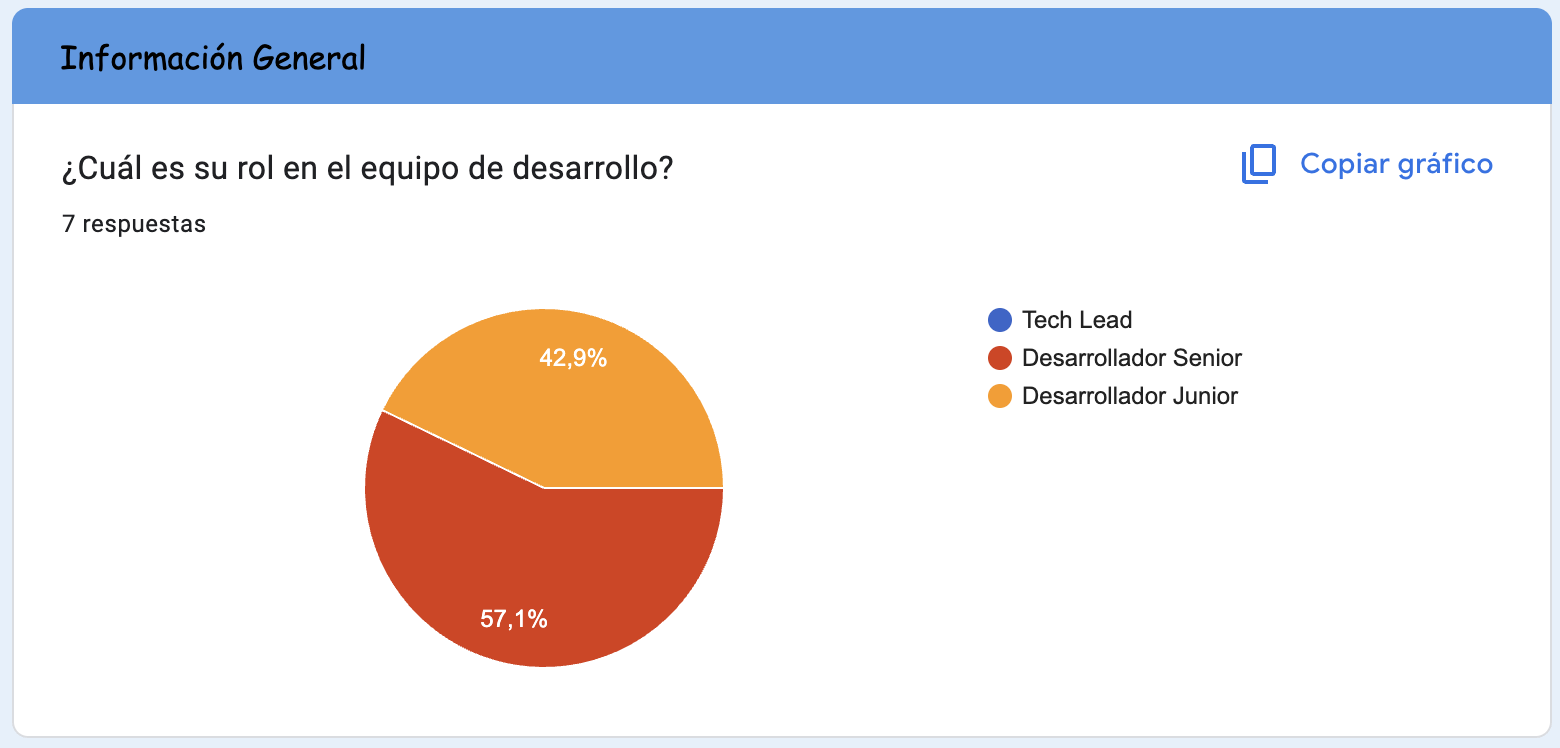
\includegraphics[width=1\textwidth]{images/question_1.png}
    \caption{Encuesta: Pregunta 1}
    \label{fig:question_1}
\end{figure}

\FloatBarrier

Esto indica que un 57 \% es desarrollador Senior, lo cual refleja que esta encuesta estará predominada por personas con bastante experiencia en el rubro de la industria del software.

\FloatBarrier
\begin{figure}[h!]
    \centering
    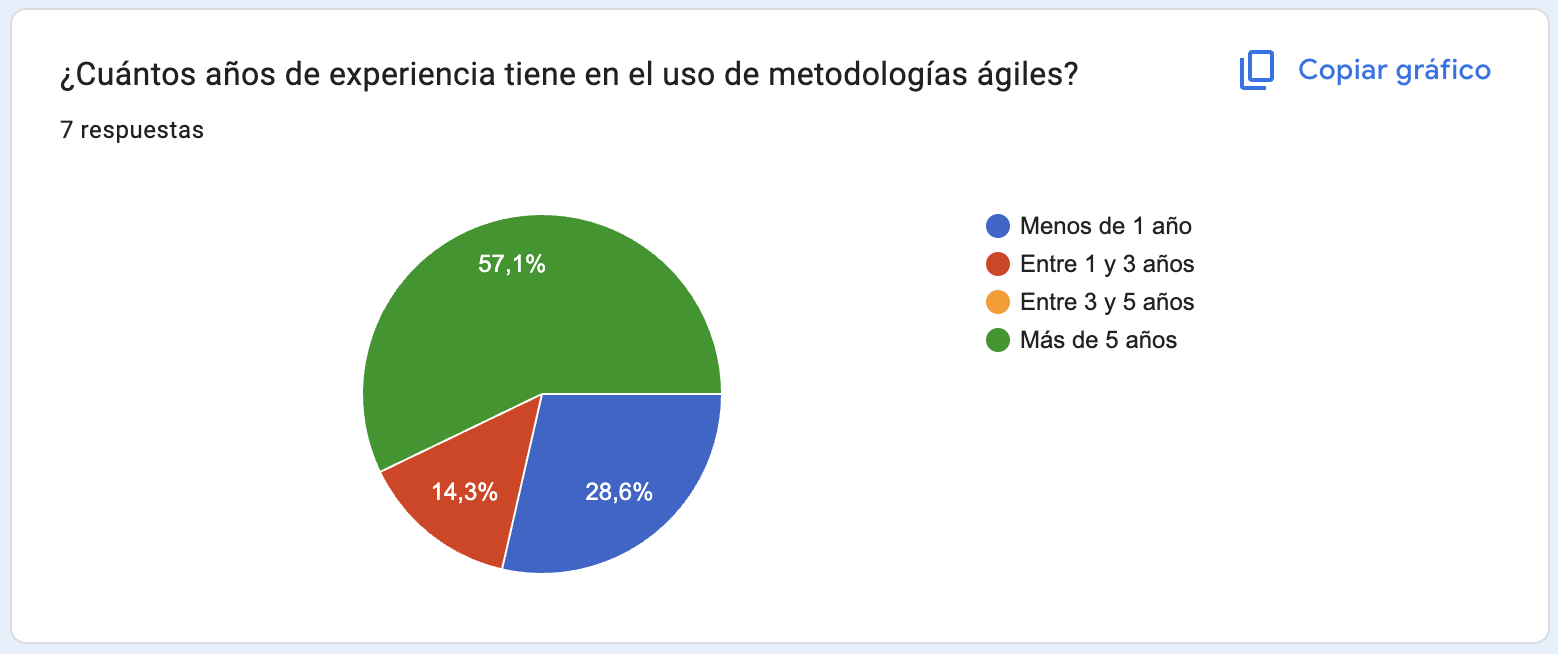
\includegraphics[width=1\textwidth]{images/question_2.png}
    \caption{Encuesta: Pregunta 2}
    \label{fig:question_2}
\end{figure}

\FloatBarrier
Esta imagen nos indica que el 57.1\% ya ha trabajado con alguna metología ágil, es decir que en sus equipos de trabajo es casi un estilo de trabajo en equipo usando estas metodologías, lo que podría reflejar que no sería difícil poder ajustarse a las empresas a ajustarse usando el mismo modelo de estimaciones, pero aplicado en los costos.


\FloatBarrier
\begin{figure}[h!]
    \centering
    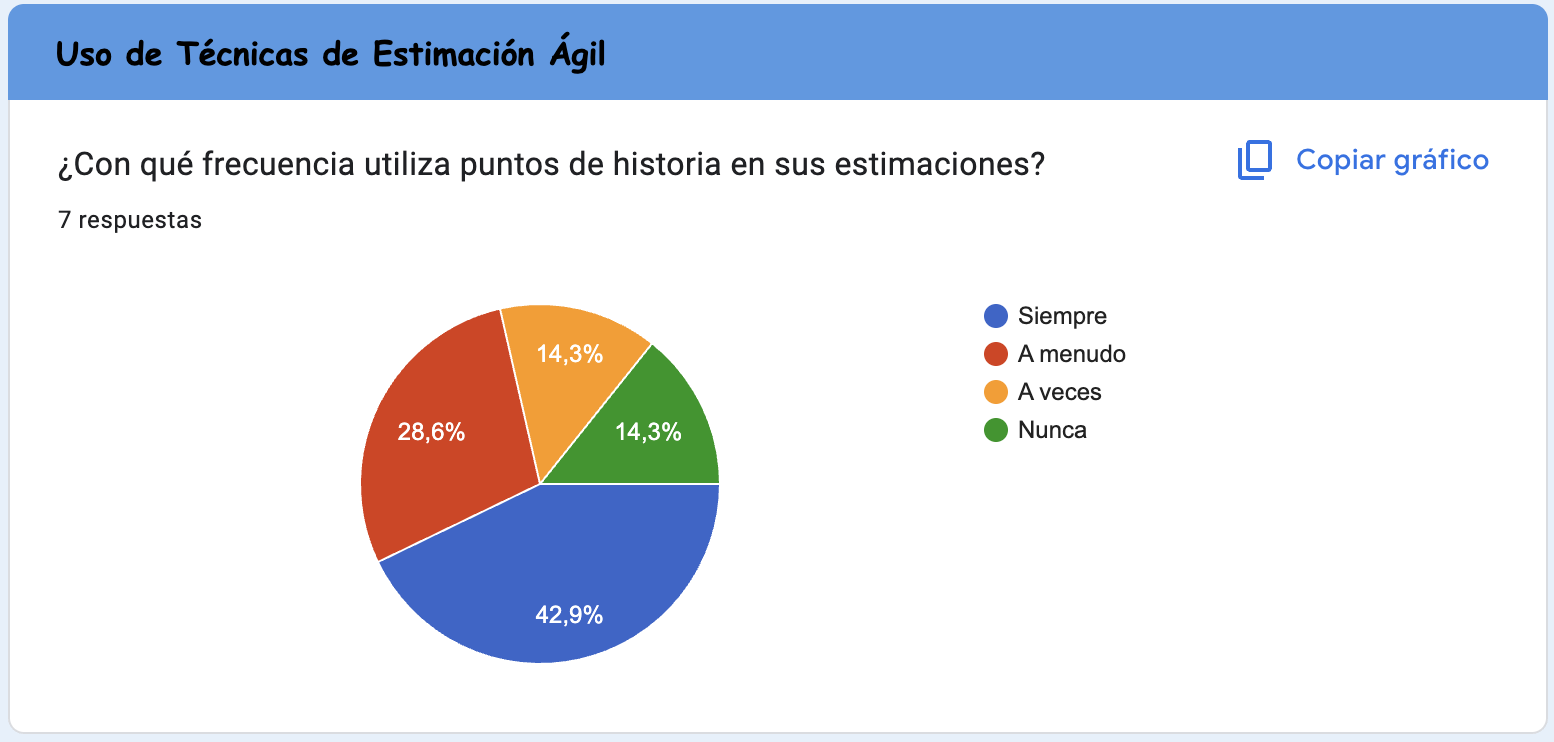
\includegraphics[width=1\textwidth]{images/question_3.png}
    \caption{Encuesta: Pregunta 3}
    \label{fig:question_3}
\end{figure}

\FloatBarrier
Este comportamiento refleja que, aunque los puntos de historia son ampliamente aceptados como una técnica ágil efectiva, existe un porcentaje considerable de equipos que no los utilizan con regularidad. Las razones pueden deberse a la falta de experiencia con metodologías ágiles, el tamaño reducido de los equipos, o la percepción de que la técnica no aporta valor en ciertos contextos específicos. Es importante analizar las barreras que limitan su adopción para proponer estrategias que promuevan su uso consistente y efectivo.

\FloatBarrier
\begin{figure}[h!]
    \centering
    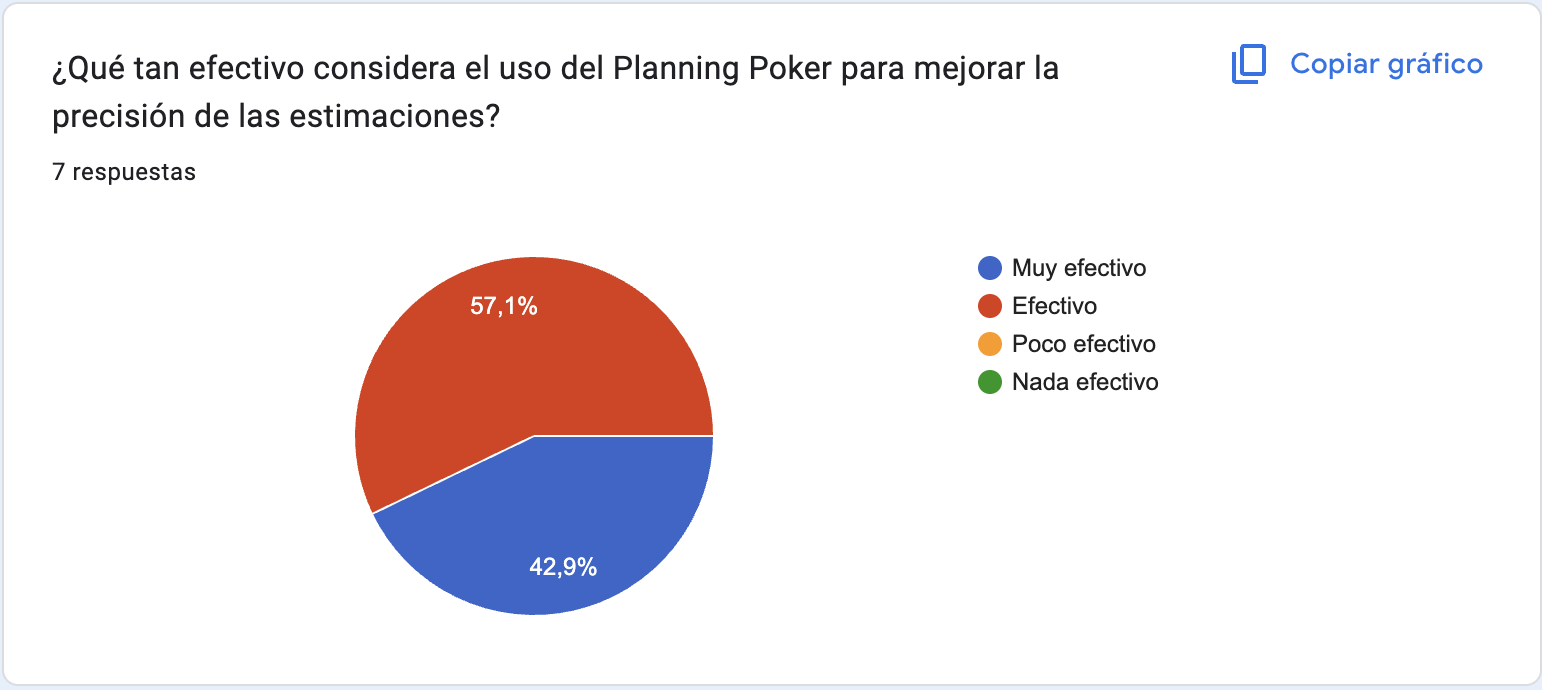
\includegraphics[width=1\textwidth]{images/question_4.png}
    \caption{Encuesta: Pregunta 4}
    \label{fig:question_4}
\end{figure}


\FloatBarrier
El gráfico ilustra la percepción de los encuestados sobre la efectividad del Planning Poker para mejorar la precisión en las estimaciones. Se observa que el 57.1\% considera esta técnica como efectiva, mientras que un 42.9\% la califica como muy efectiva.

Estos resultados reflejan un alto nivel de aceptación de Planning Poker dentro de los equipos de desarrollo, confirmando su utilidad como herramienta colaborativa para alcanzar estimaciones más precisas. La participación activa de los miembros del equipo en el proceso fomenta el consenso y permite ajustar las percepciones individuales, reduciendo la incertidumbre y mejorando la calidad de las proyecciones. Sin embargo, la ausencia de respuestas negativas (poco efectivo o nada efectivo) indica que, en los equipos evaluados, Planning Poker se ha consolidado como una práctica eficiente y valorada en contextos ágiles.

\FloatBarrier
\begin{figure}[h!]
    \centering
    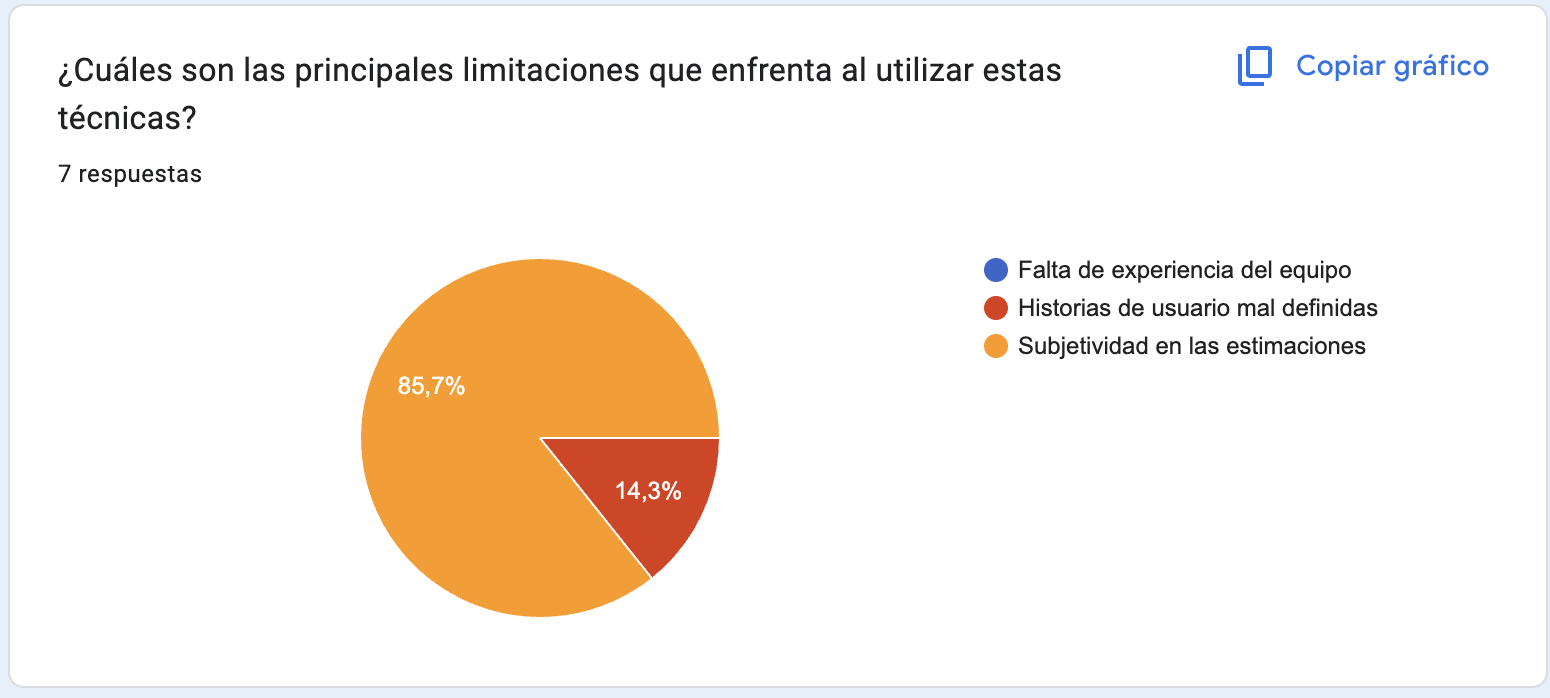
\includegraphics[width=1\textwidth]{images/question_5.png}
    \caption{Encuesta: Pregunta 5}
    \label{fig:question_5}
\end{figure}


\FloatBarrier
Es relevante destacar que no se mencionó la falta de experiencia del equipo como una limitación, lo cual sugiere que los participantes cuentan con un nivel adecuado de conocimiento en metodologías ágiles. Sin embargo, los resultados subrayan la necesidad de implementar prácticas que reduzcan la subjetividad en las estimaciones, como el uso de datos históricos, métricas más objetivas y un mejor refinamiento de las historias de usuario.

\section{Conclusiones Generales}
El presente análisis sobre la estimación de costos en el desarrollo de software utilizando enfoques ágiles, como los puntos de historia y el Planning Poker, permite identificar tanto la aceptación como los desafíos asociados a estas técnicas dentro de los equipos de desarrollo.

En primer lugar, los resultados muestran que un 42.9\% de los encuestados utiliza los puntos de historia de manera constante, lo que refleja una alta adopción de esta herramienta como método principal de estimación en equipos ágiles. Sin embargo, un 28.6\% lo usa con menos frecuencia, lo que podría indicar variabilidad en su implementación dependiendo del contexto o de la experiencia del equipo.

En relación con el Planning Poker, la técnica es percibida positivamente, con un 57.1\% calificándola como efectiva y un 42.9\% como muy efectiva. Esta evaluación confirma la utilidad de Planning Poker como una herramienta colaborativa para mejorar la precisión de las estimaciones, especialmente al fomentar la participación del equipo y alcanzar consensos.

Por otro lado, se evidencian limitaciones importantes en el uso de estas técnicas. La subjetividad en las estimaciones fue identificada como el principal desafío por el 85.7\% de los encuestados, lo que subraya la necesidad de minimizar la variabilidad mediante mejores prácticas y herramientas complementarias. Adicionalmente, un 14.3\% señaló las historias de usuario mal definidas como una barrera significativa, lo que destaca la importancia de contar con requerimientos claros y bien estructurados para obtener estimaciones más precisas.

En conclusión, aunque las técnicas de puntos de historia y Planning Poker son valoradas positivamente y ampliamente adoptadas, su efectividad depende en gran medida de factores como la claridad de los requerimientos, la experiencia del equipo y la implementación de mecanismos que reduzcan la subjetividad. Es necesario fomentar un proceso más riguroso de definición de historias de usuario y explorar el uso de datos históricos o herramientas de análisis predictivo para mejorar la objetividad y consistencia de las estimaciones en proyectos ágiles de desarrollo de software.
\chapter{Recomendaciones}

\section{Resumen}
En función de los hallazgos obtenidos en el análisis, se proponen las siguientes recomendaciones para optimizar el uso de \textit{puntos de historia} y \textit{Planning Poker} como técnicas de estimación de costos en proyectos de desarrollo de software:

\begin{enumerate}
    \item \textbf{Refinamiento de Historias de Usuario:}
    \begin{itemize}
        \item Implementar sesiones de refinamiento de historias de usuario antes del proceso de estimación, asegurando que los requerimientos sean claros, precisos y desglosados.
        \item Utilizar criterios como \textit{INVEST} (Independiente, Negociable, Valiosa, Estimable, Pequeña y Verificable) para mejorar la calidad de las historias de usuario.
    \end{itemize}

    \item \textbf{Capacitación del Equipo:}
    \begin{itemize}
        \item Realizar capacitaciones periódicas sobre metodologías ágiles y buenas prácticas de estimación para asegurar la correcta aplicación de las técnicas.
        \item Promover ejercicios de estimación en equipos heterogéneos, facilitando la objetividad y el aprendizaje compartido.
    \end{itemize}

    \item \textbf{Uso de Datos Históricos:}
    \begin{itemize}
        \item Incorporar el uso de datos históricos y métricas cuantitativas, como la velocidad del equipo, para validar y ajustar las estimaciones.
        \item Utilizar herramientas de gestión como \textit{Jira} o \textit{Trello} para almacenar y analizar patrones de desempeño.
    \end{itemize}

    \item \textbf{Reducción de la Subjetividad:}
    \begin{itemize}
        \item Fomentar la participación equitativa durante el \textit{Planning Poker} para evitar la influencia de opiniones dominantes.
        \item Complementar el \textit{Planning Poker} con técnicas alternativas, como la estimación por rangos o el uso de puntos de confianza.
    \end{itemize}

    \item \textbf{Monitoreo y Retroalimentación Continua:}
    \begin{itemize}
        \item Implementar un proceso de revisión al final de cada iteración, comparando las estimaciones iniciales con el esfuerzo real.
        \item Fomentar la retroalimentación constante para identificar dificultades y mejorar la aplicación de estas técnicas.
    \end{itemize}

    \item \textbf{Adopción de Herramientas Tecnológicas:}
    \begin{itemize}
        \item Incorporar herramientas tecnológicas como \textit{Jira}, \textit{Monday.com} o \textit{Azure DevOps} para facilitar el seguimiento y análisis de las estimaciones.
    \end{itemize}
\end{enumerate}

Estas recomendaciones están orientadas a reducir las limitaciones observadas, como la subjetividad en las estimaciones y las historias de usuario mal definidas, mejorando así la precisión y efectividad de las técnicas ágiles de estimación en proyectos de desarrollo de software.

\appendix
\chapter{Anexo: Encuesta sobre Técnicas de Estimación Ágil}
\section*{Sección: Información General}
\begin{enumerate}
    \item ¿Cuál es su rol en el equipo de desarrollo?
    \begin{enumerate}
        \item Tech Lead
        \item Desarrollador Senior
        \item Desarrollador Junior
        \item Otro
    \end{enumerate}
    \item ¿Cuántos años de experiencia tiene en el uso de metodologías ágiles?
    \begin{enumerate}
        \item Menos de 1 año
        \item Entre 1 y 3 años
        \item Entre 3 y 5 años
        \item Más de 5 años
    \end{enumerate}
\end{enumerate}

\section*{Sección: Uso de Técnicas de Estimación Ágil}
\begin{enumerate}[resume]
    \item ¿Con qué frecuencia utiliza puntos de historia en sus estimaciones?
    \begin{enumerate}
        \item Siempre
        \item A menudo
        \item A veces
        \item Nunca
    \end{enumerate}
    \item ¿Qué tan efectivo considera el uso del Planning Poker para mejorar la precisión de las estimaciones?
    \begin{enumerate}
        \item Muy efectivo
        \item Efectivo
        \item Poco efectivo
        \item Nada efectivo
    \end{enumerate}
    \item ¿Cuáles son las principales limitaciones que enfrenta al utilizar estas técnicas?
    \begin{enumerate}
        \item Falta de experiencia del equipo
        \item Historias de usuario mal definidas
        \item Subjetividad en las estimaciones
        \item Otro
    \end{enumerate}
\end{enumerate}


\newpage
\printbibliography

\end{document}
